\subsection{Auslesen des Framebuffer}
Einer der ersten Schritte, die ein Angreifer nach Erlangen einer Shell durchführt, ist die Abfrage der User-ID über \texttt{id}.
Der Befehl zeigt an, dass der eingeloggte \texttt{bastion}-Benutzer Teil der \texttt{video}-Gruppe ist, die unter anderem das Lesen des Bildschirminhalts erlaubt.

Der Framebuffer kann über die Datei \texttt{/dev/fb0} ausgelesen und auf die eigene Maschine kopiert werden:
\begin{lstlisting}
ssh bastion@localhost "cat /dev/fb0" > fb0.raw
\end{lstlisting}

Anders als etwa JPEG- oder PNG-Bilder wird der Framebuffer nicht komprimiert gespeichert, sondern enthält Pixel für Pixel die einzelnen Werte für die Farbkanäle.
Ferner bedeutet das auch, dass die Auflösung nicht in der Datei enthalten ist.

An dieser Stelle kann die Auflösung entweder durch ausprobieren, durch Berechnungen auf Basis der Dateigröße oder mit dem Befehl \texttt{fbset} ermittelt werden:
\begin{itemize}
\item In den ersten beiden Fällen muss nur die Weite des Bildschirms geraten werden und die Höhe ergibt sich automatisch. Der Framebuffer ist etwa 1572864~Bytes groß, bei 16-bit Farbtiefe (das ist üblich bei Framebuffern) sind das 786432~Pixel. Mit der gerateten Weite von 1024~Pixeln ergibt sich eine Höhe von 786432 / 1024 = 768~Pixeln.
\item Im letzten Fall gibt \texttt{fbset} sowohl die Bildschirmgröße als auch die Kodierung zurück:
\begin{lstlisting}
mode "1024x768-0"
	# D: 0.000 MHz, H: 0.000 kHz, V: 0.000 Hz
	geometry 1024 768 1024 768 32
	timings 0 0 0 0 0 0 0
	accel true
	rgba 8/16,8/8,8/0,0/0
endmode
\end{lstlisting}
\end{itemize}

Um den Framebuffer nun sichtbar zu machen, bietet sich GIMP an, das bereits eine Funktion zum Lesen roher Bilddaten enthält.
Über eine schnelle Google-Suche sind allerdings auch einige fertige Python-Skripte zu finden, die den Framebuffer in eine PNG umwandeln können.

\begin{figure}[!ht]
\centering
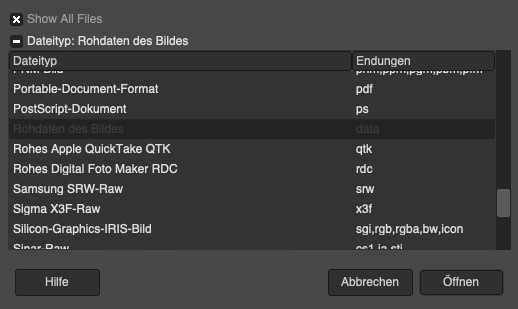
\includegraphics[width=.7\textwidth]{img/video_gimp_open.png}
\caption{Öffnen des Framebuffer als rohes Bild in GIMP}
\end{figure}

In einem neuen Fenster ist dann eine Vorschau des Framebuffer zu sehen, hier müssen jedoch noch die Dimensionen und die Kodierung spezifiziert werden.
Wenn noch nicht erfolgt, dann kann auch über das Vorschaufenster die Bildschirmgröße geraten bzw. ausprobiert werden.

\begin{figure}[!ht]
\centering
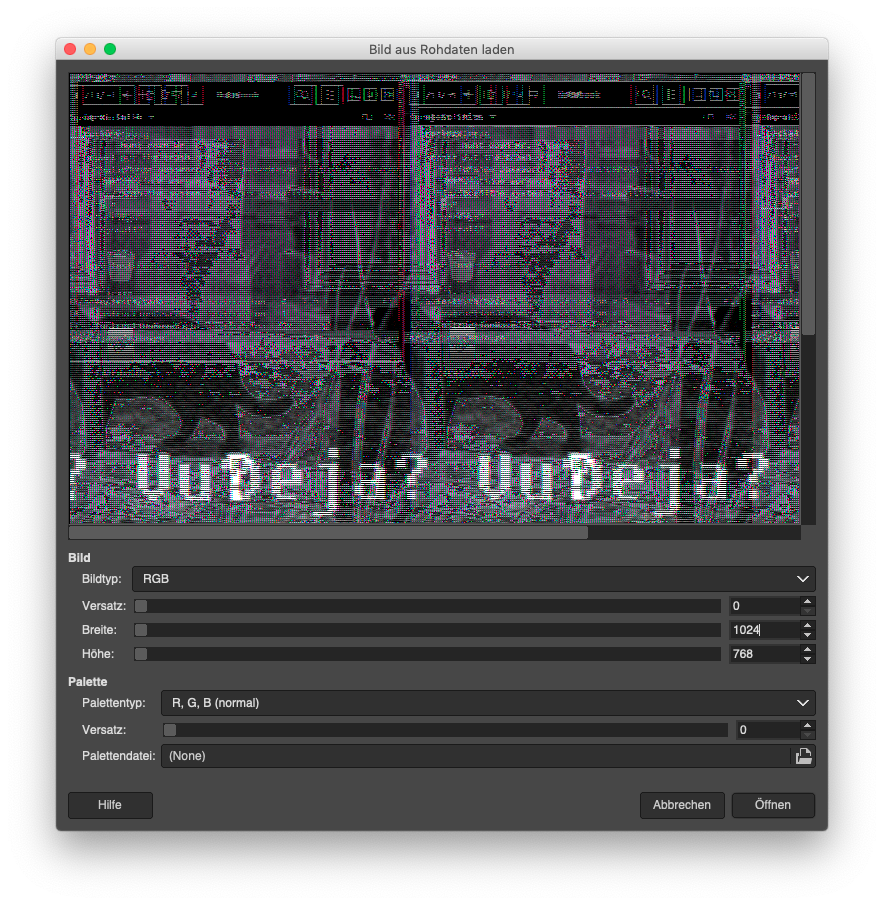
\includegraphics[width=\textwidth]{img/video_gimp_load.png}
\caption{Vorschau des Framebuffer}
\label{fig:video_gimp_load}
\end{figure}

In \cref{fig:video_gimp_load} wurde der Bildtyp bzw. die Kodierung noch nicht korrekt ausgewählt.
Hier kann auch entweder kurz durchprobiert oder die Kodierung aus \texttt{fbset} gelesen werden.
Häufig sind Framebuffer in RGB565 kodiert, wie auch hier, in diesem Fall in Little-Endian.

\clearpage
\begin{landscape}
\begin{figure}[!ht]
\centering
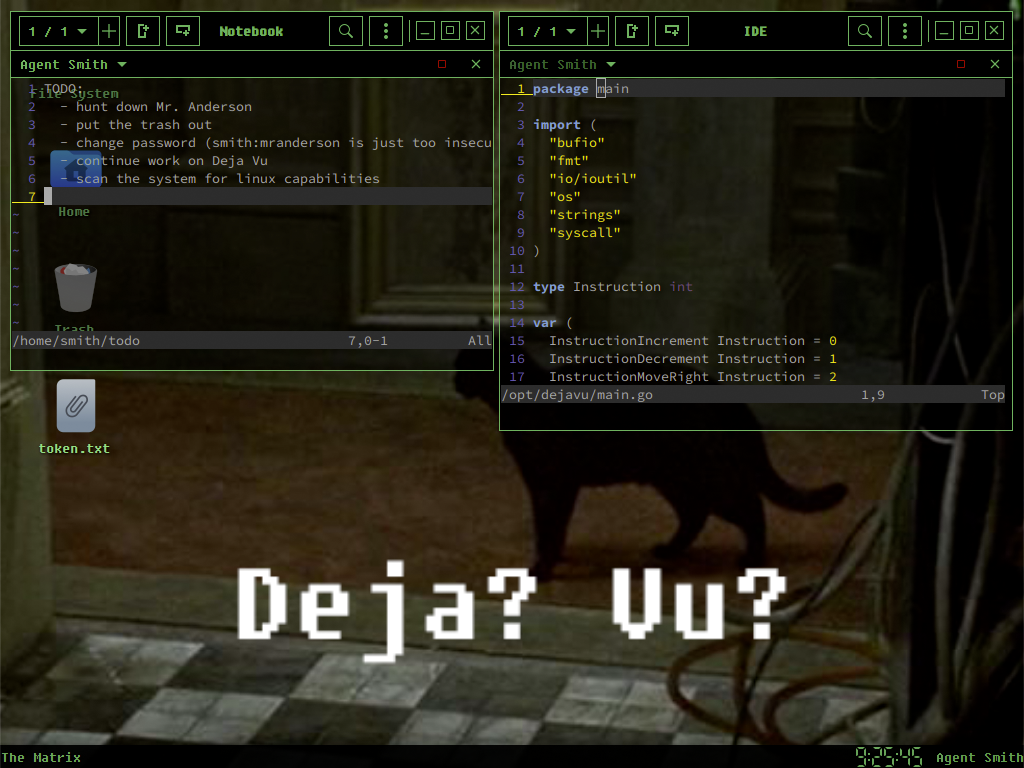
\includegraphics[height=\textwidth]{video/fb0.png}
\caption{Der Bildschirm, wie er im Framebuffer gespeichert ist}
\end{figure}
\end{landscape}
\clearpage

Prinzipiell wurde in dem Schritt also ein Screenshot gemacht, auf dem nun zu sehen ist, dass Agent~Smith eingeloggt ist.
Des Weiteren ist eine TODO-Liste geöffnet sowie der Quellcode von einem Programm.

Aus der TODO-Liste lässt sich ermitteln, dass Agent~Smith den Benutzernamen \texttt{smith} und das Passwort \texttt{mranderson} hat.

Im Screenshot finden sich weitere Hinweise (\enquote{Deja Vu} im TODO und Hintergrund sowie im Quellcode, Linux Capabilities), die aber erst für spätere Schritt interessant sind.

In einer neuen SSH Sitzung kann sich nun als Benutzer \texttt{smith} mit genanntem Passwort eingeloggt werden.
Die \texttt{/home/smith/Desktop/token.txt} enthält das folgende Token:
\lstinputlisting{tokens/token2}
